\clearpage
\section{Discussion}
\label{sec:methods-discussion}
%%%%%

\info[inline]{Paragraph: Discuss relevant topics before starting the benchmarking chapter.}
Here we briefly discuss any remaining issues and considerations regarding methods development.

%%
\subsection{Model-based and data-driven methods}
\label{subsec:model-based-data-driven-methods}
%%

\info[inline]{Paragraph: Discuss benefits of model-based approaches.}
Model-based approaches have multiple benefits over descriptive methods such as \gls{sw} approaches~\parencite{Foti2019}.
Models of the underlying process have increased predictive power, which has long been argued to be essential to true understanding of \gls{fc}~\parencite{Bassett2011}.
They also allow for easier specification of inductive biases.
They naturally deal with sparse and missing data regimes.
Furthermore, they allow for model synchronization, where various smaller models can be combined, or side information can be included.
As such, everything else being equal we should prefer model-based approaches for \gls{tvfc} estimation.
%
In terms of model selection, all estimation methods described have parameters that need to be chosen or tuned.
This does mean that more complex models with more parameters to tune come with a complexity penalty~\parencite[see also][]{Sculley2015}.
Here we discuss several more considerations regarding model-based and data-driven approaches.

%%
\subsubsection{Uncertainty and interpretability}
%%

The \gls{wp} model may lead to improved performance, flexibility, and interpretability.
Additionally, we can sample our covariance matrix at any point in time, and get uncertainty in our estimates (unlike the other methods discussed).
The importance of uncertainty in covariance estimates has been discussed by~\textcite{Kudela2017}.
Under a fully probabilistic model, it is also easier to do hypothesis tests whether there is any \gls{tvfc} present at all.

%%
\subsubsection{Artifacts and asynchronous data}
%%

The \gls{wp} approach allows a practitioner to drop out certain data points.
This can be useful for neuroimaging data, as measurement artifacts can elegantly be left out.
All artifacts and limitations of \gls{fmri} data are directly relevant to any \gls{tvfc} analysis as well~\parencite{Nalci2019}.
For example, outliers due to head motion can have a large impact on the signal~\parencite{Power2014, Power2015}.
Current popular methods do not allow for this, and would typically need to interpolate the missing values.
%
Although it seems that we still need all $D$ points to be present for $Y_n$, this can be mitigated.
We can add infinite noise to a data point so that it does not affect the posterior.
Thus, this model can accept asynchronous data.

The steps taken to process neuroimaging data are under heavy debate~\parencite[see e.g.][]{Poldrack2017, Botvinik-Nezer2020, Lindquist2020, Elliott2021}.
Certain steps are included to get the data into a format that current covariance models expect.
When we use a more flexible model such as the \gls{wp}, this may affect what steps to include and how data is processed.
For example, since we can operate on asynchronous data, slice timing correction may not be needed anymore.
This highlights the benefits of viewing preprocessing and analysis as a joint, interweaved process instead of two separate steps.

%%
\subsection{Higher dimensions: Pairwise or joint modeling?}
\label{subsec:higher-dimensions}
%%

\info[inline]{Paragraph: Discuss the issue of pairwise or joint modeling.}
When we are faced with the case of $D > 2$, we can either opt for modeling the covariance structure of all time series jointly, or for looping over all pairs of time series (training $\frac{D (D - 1)}{2}$ models instead).
%
For example, \textcite{Choe2017, Hakimdavoodi2020} chose for the latter when implementing \gls{dcc}.
This may be due to \gls{mgarch} models having a reputation for not scaling well to higher dimensions.
%
What is the difference between these two options?
And how does this relate to multiple hypothesis testing?
First of all, \gls{sw} approaches are always pairwise.
However, the window length and other global parameters operate on all edges.
As a fair comparison to this standard approach, training the \gls{wp} and \gls{dcc} models in multivariate (joint) fashion is the fairest comparison.
Even if we determine the window length from the data using \gls{sw-cv}, we have to choose whether to use the same window length for all edges, or a different one for each edge.
%
Whether it is relevant to learn different hyperparameters for each edge (or node) really depends on whether we expect significantly different dynamic characteristics between edges (and nodes).
For example, a certain edge's connectivity may be static across time, whereas another changes rapidly (simulated in \cref{fig:pairwise-vs-joint}).
%
Secondly, if a method outperforms the others consistently in the bivariate ($D = 2$) case, it should also outperform if we choose to loop over all edges.
This means that if we plan to only train pairwise models, we need only compare methods on the bivariate case.


\begin{figure}[t]
  \centering
  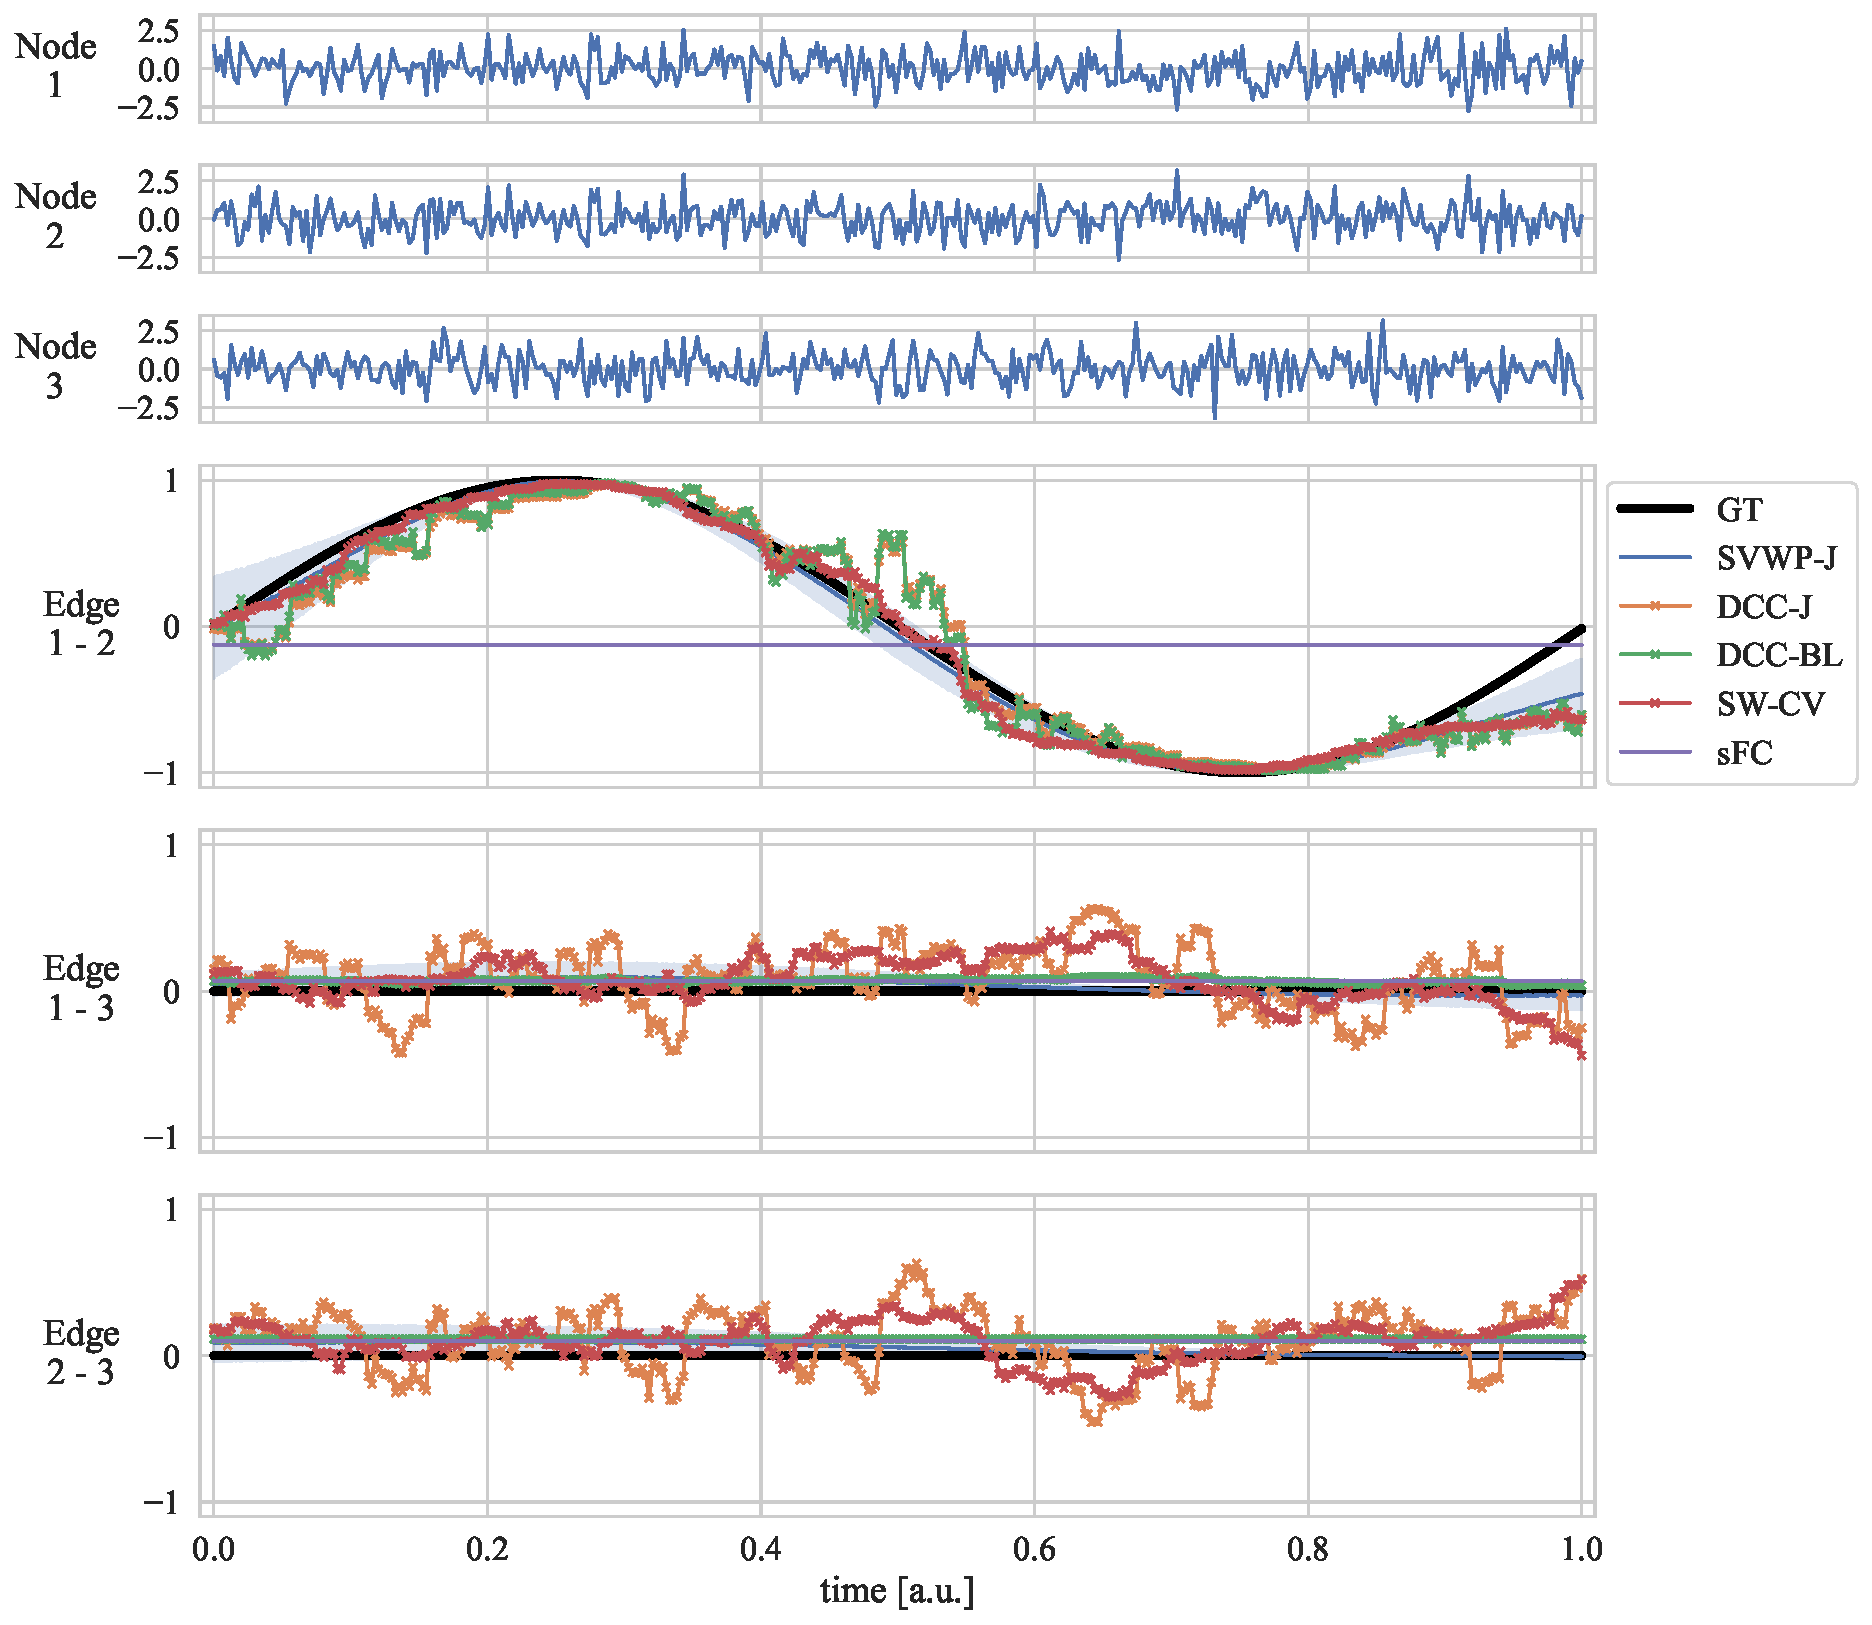
\includegraphics[width=\textwidth]{fig/sim/d3s/N0400_T0003/no_noise/periodic_1_correlations}
  \caption{
    Demonstration and motivation for training models in pairwise fashion when edges are characterized by radically different covariance structures.
  }
  \label{fig:pairwise-vs-joint}
\end{figure}


\info[inline]{Paragraph: Discuss our approach to this issue.}
In a theoretical approach, in general, a model should expect to always find some pair that seems correlated when presented with a large number of pairs.
A multivariate model would not extract spurious structure if it only sees one odd case out of many, or at least would need even more evidence.
However, the pairwise approach would not have this inherent protection against reporting false positives.
Of course, such issues could be resolved through careful post-estimation multiple comparison correction.
%
On the other hand, in an empirical approach, we can also directly compare both implementations (joint and pairwise loop) and check which one performs better on the benchmarks.
In fact, this is one of the strengths of properly designed benchmarks: it reduces speculation.
For example, \cref{fig:pairwise-vs-joint} shows \gls{tvfc} estimates for a toy example of $D = 3$ simulated time series, where the first two nodes exhibit a periodic covariance structure and the other edges are uncorrelated.
The pairwise \gls{dcc} model predicts better than the jointly trained \gls{dcc} model, arguably because the covariance structure characteristics are radically different for the different edges.
This seems to motivate the benefit of training \gls{dcc} in a pairwise fashion.
However, as we shall see later, in realistic scenarios these differences will not be as pronounced, and the two ways of training yield very similar estimates.
%
Throughout this thesis we train all models in joint fashion, except \gls{dcc} which will be trained in both manners.
The `-J' suffix will indicate a multivariate jointly trained model, where `-BL' will refer to bivariate (pairwise) loop training.
For the bivariate case, this distinction becomes meaningless, and the suffixes are dropped.

%%
\subsection{Autoregressive and full process dependence}
%%

Estimation methods can broadly be divided into constructions that are autoregressive (taking only past observations into account) in nature or that depend on the full process.
%
\Glspl{gp} assume full process dependence, so our \gls{wp} follows suite.
Methods based on \gls{sw} fall into this category as well.
%
However, the \gls{dcc} method does not, and in their introductory paper \textcite{Lindquist2014} designed their \gls{sw} methods to only incorporate past data to allow for a fair comparison.
Training \gls{dcc} models does involve tuning hyperparameters, however, which are learned based on the full time series.
%
In this thesis we argue that forecasting is typically not of major interest in neuroimaging, and that full scans are always available at analysis time.
Therefore, we do not make a distinction between such models, and compare them head-to-head.

%%
\subsection{Beyond simple performance metrics}
%%

\info[inline]{Paragraph: Discuss other key motivations when choosing a TVFC estimation method.}
While a carefully designed benchmark and performance metric should provide guidance on what methods perform best, there are other method qualities that are desirable.
%
These include computational complexity, uncertainty modeling and estimation, robustness, ease of implementation, explainability, and flexibility in general.
%
These will be considered secondary (or \emph{auxiliary}) factors in our model comparison.
For example, it seems reasonable to want to sacrifice on performance slightly if it would get you many other attractive characteristics in return.
%
We will return to this in \cref{ch:discussion}.

%%
\subsection{Other benchmarks}
%%

\info[inline]{Paragraph: Discuss other benchmarks not included here and what we miss out on.}
The families of benchmarks discussed in this chapter are not exhaustive.
%
Other benchmarks outside the scope of this thesis include predicting a concurrent modality.
For example, by using a simultaneous \gls{fmri}-\gls{eeg} data set~\parencite{Laufs2003}.
\textcite{Tagliazucchi2014} predicted sleep state from \gls{fmri} using such a concurrent data set.
Other concurrent modalities are possible as well.
For example, \textcite{Matsui2016} simultaneously monitored neuronal calcium signals and \gls{fmri}.
%
The problem with such data sets is often that they are hard to process and understand, and they may not make for practically useful benchmarking data sets at the moment.
This leads to typically sample sizes too.
